  
\documentclass[12pt,a4paper,fleqn]{tufte-handout} 
\usepackage{graphicx} 
\usepackage{morefloats} 
\usepackage{amsmath} 
\usepackage{amssymb} 
\usepackage{rotating} 
% mcode options for matlab code insertion bw (for printing), numbered (line numbers), framed (frame around code blocks), useliterate (convert Matlab expressions to Latex ones), autolinebreaks (automatic code wraping, use it with caution 
\usepackage[literate]{mcode} 
\graphicspath{{figures/}{tex/}{../figures/}{../../}{../}}  
\title{mkaTimeSeriesPaper} 
\author{ Mathieu Lagrange } 
  
\begin{document} 
  
\maketitle 
  
% Please use this file to document your experiment 
% You can compile the report by setting the option 'report' as detailed in your expCode configuration file. 
  
  
  
 
  
  
\begin{center} 
  
  
\begin{figure} 
  
  
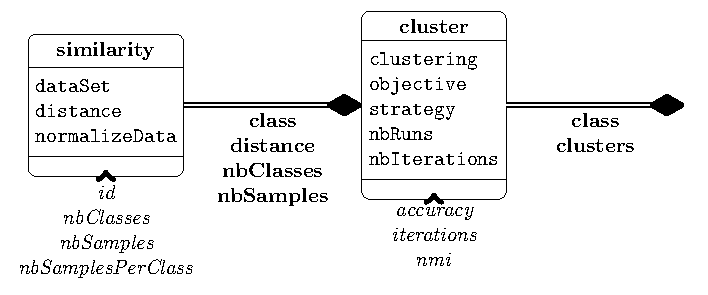
\includegraphics[width=\textwidth,height=0.8\textheight,keepaspectratio]{../figures/factors.pdf} 
  
  
\label{factorFlowGraph} 
  
  
\caption{Factors flow graph for the experiment.} 
  
  
\end{figure} 
  
  
\end{center} 
  
  
\begin{table} 
\begin{center} 
\ 
 \setlength{\tabcolsep}{.16667em} 
\begin{tabular}{lc} 
dataSet & id \\ 
\hline 
50words &  1 \\ 
Adiac &  2 \\ 
Beef &  3 \\ 
CBF &  4 \\ 
ChlorineConcentration &  5 \\ 
CinC\_ECG\_torso &  6 \\ 
Coffee &  7 \\ 
Cricket\_X &  8 \\ 
Cricket\_Y &  9 \\ 
Cricket\_Z & 10 \\ 
DiatomSizeReduction & 11 \\ 
ECG200 & 12 \\ 
ECGFiveDays & 13 \\ 
FaceAll & 14 \\ 
FaceFour & 15 \\ 
FacesUCR & 16 \\ 
Gun\_Point & 17 \\ 
Haptics & 18 \\ 
InlineSkate & 19 \\ 
ItalyPowerDemand & 20 \\ 
Lighting2 & 21 \\ 
Lighting7 & 22 \\ 
MALLAT & 23 \\ 
MedicalImages & 24 \\ 
MoteStrain & 25 \\ 
OSULeaf & 26 \\ 
OliveOil & 27 \\ 
SonyAIBORobotSurface & 28 \\ 
SonyAIBORobotSurfaceII & 29 \\ 
StarLightCurves & 30 \\ 
SwedishLeaf & 31 \\ 
Symbols & 32 \\ 
Trace & 33 \\ 
TwoLeadECG & 34 \\ 
Two\_Patterns & 35 \\ 
WordsSynonyms & 36 \\ 
fish & 37 \\ 
synthetic\_control & 38 \\ 
uWaveGestureLibrary\_X & 39 \\ 
uWaveGestureLibrary\_Y & 40 \\ 
uWaveGestureLibrary\_Z & 41 \\ 
wafer & 42 \\ 
yoga & 43 \\ 
\end{tabular} 
\end{center} 
\caption{normalizeData: 1} 
\label{noda1} 
\end{table} 
 
  
\begin{table} 
\begin{center} 
\ 
 \setlength{\tabcolsep}{.16667em} 
\begin{tabular}{lcc} 
id & nbClasses & nbSamplesPerClass \\ 
\hline 
 7 & 2 &      28$\pm$1 \\ 
12 & 2 &    100$\pm$47 \\ 
13 & 2 &     442$\pm$0 \\ 
17 & 2 &     100$\pm$0 \\ 
20 & 2 &     548$\pm$1 \\ 
21 & 2 &     60$\pm$18 \\ 
25 & 2 &    636$\pm$69 \\ 
28 & 2 &    310$\pm$54 \\ 
29 & 2 &   490$\pm$161 \\ 
34 & 2 &     581$\pm$0 \\ 
42 & 2 & 3582$\pm$3988 \\ 
43 & 2 &  1650$\pm$170 \\ 
\end{tabular} 
\end{center} 
\caption{Morphology of the datasets} 
\label{didtNoda1} 
\end{table} 
 
  
\begin{table} 
\begin{center} 
\small 
 \setlength{\tabcolsep}{.16667em} 
\begin{tabular}{lllccccccccc} 
 &  &  &  &  &  & kMeans & kkMeans & kAverages & kAverages & kAverages & kAverages \\ 
\hline 
 &  &  &  &  &  &  &  & object & raw & object & raw \\ 
 &  &  & id & nbClasses & nbSamplesPerClass &  &  & p & p & b & b \\ 
 &  &  &  7 & 2 &      28$\pm$1 & 48$\pm$12 & \textbf{48$\pm$32} & \textbf{54$\pm$26} & \textbf{\textcolor{red}{66$\pm$32}} & \textbf{48$\pm$26} & \textbf{51$\pm$37} \\ 
 &  &  & 12 & 2 &    100$\pm$47 & 12$\pm$2 & 14$\pm$3 & \textbf{\textcolor{red}{15$\pm$0}} & 10$\pm$5 & \textbf{\textcolor{red}{15$\pm$0}} & 10$\pm$5 \\ 
 &  &  & 13 & 2 &     442$\pm$0 &  0$\pm$0 &  2$\pm$2 & \textbf{ 4$\pm$6} & \textbf{ 5$\pm$2} & \textbf{\textcolor{red}{9$\pm$12}} & \textbf{ 5$\pm$2} \\ 
 &  &  & 17 & 2 &     100$\pm$0 & 0 & 0 & 0 & \textbf{1} & 0 & \textbf{\textcolor{red}{1}} \\ 
 &  &  & 20 & 2 &     548$\pm$1 & \textbf{0$\pm$0} & \textbf{1$\pm$0} & \textbf{0$\pm$0} & \textbf{1$\pm$0} & \textbf{\textcolor{red}{1$\pm$5}} & \textbf{1$\pm$0} \\ 
 &  &  & 21 & 2 &     60$\pm$18 & \textbf{3$\pm$0} & 1$\pm$0 & 1$\pm$0 & \textbf{3$\pm$4} & 1$\pm$0 & \textbf{\textcolor{red}{4$\pm$4}} \\ 
 &  &  & 25 & 2 &    636$\pm$69 & 30$\pm$0 & \textbf{\textcolor{red}{52$\pm$0}} & 41$\pm$0 & 36$\pm$1 & 41$\pm$0 & 36$\pm$1 \\ 
 &  &  & 28 & 2 &    310$\pm$54 & 55$\pm$21 & \textbf{\textcolor{red}{ 78$\pm$0}} &  72$\pm$1 &  21$\pm$0 &  72$\pm$1 &  21$\pm$0 \\ 
 &  &  & 29 & 2 &   490$\pm$161 & \textbf{\textcolor{red}{24}} & 21 & 22 & 15 & 22 & 15 \\ 
 &  &  & 34 & 2 &     581$\pm$0 & 0$\pm$0 & 7$\pm$0 & 7$\pm$0 & \textbf{\textcolor{red}{8$\pm$0}} & 7$\pm$0 & \textbf{\textcolor{red}{8$\pm$0}} \\ 
 &  &  & 42 & 2 & 3582$\pm$3988 & \textbf{\textcolor{red}{0}} & 0 & 0 & 0 & 0 & 0 \\ 
 &  &  & 43 & 2 &  1650$\pm$170 & 0$\pm$0 & \textbf{\textcolor{red}{0$\pm$0}} & \textbf{0$\pm$0} & 0$\pm$0 & \textbf{0$\pm$0} & 0$\pm$0 \\ 
\end{tabular} 
\end{center} 
\caption{nbIterations: 200, distance: dtw, normalizeData: 1, nbRuns: 20} 
\label{nbit200DidtNoda1Nbru20} 
\end{table} 
 
  
\begin{table} 
\begin{center} 
\ 
 \setlength{\tabcolsep}{.16667em} 
\begin{tabular}{lcc} 
id & nbClasses & nbSamplesPerClass \\ 
\hline 
 3 & 5 &      12$\pm$0 \\ 
 4 & 3 &     310$\pm$0 \\ 
 5 & 3 &  1436$\pm$755 \\ 
 6 & 4 &     355$\pm$0 \\ 
11 & 4 &     80$\pm$31 \\ 
15 & 4 &      28$\pm$5 \\ 
18 & 5 &      93$\pm$9 \\ 
19 & 7 &     93$\pm$22 \\ 
22 & 7 &      20$\pm$8 \\ 
26 & 6 &     74$\pm$20 \\ 
27 & 4 &      15$\pm$8 \\ 
30 & 3 & 3079$\pm$2045 \\ 
32 & 6 &     170$\pm$9 \\ 
33 & 4 &      50$\pm$0 \\ 
35 & 4 &   1250$\pm$43 \\ 
37 & 7 &      50$\pm$0 \\ 
38 & 6 &     100$\pm$0 \\ 
\end{tabular} 
\end{center} 
\caption{Morphology of the datasets} 
\label{didtNoda1} 
\end{table} 
 
  
\begin{table} 
\begin{center} 
\small 
 \setlength{\tabcolsep}{.16667em} 
\begin{tabular}{lllccccccccc} 
 &  &  &  &  &  & kMeans & kkMeans & kAverages & kAverages & kAverages & kAverages \\ 
\hline 
 &  &  &  &  &  &  &  & object & raw & object & raw \\ 
 &  &  & id & nbClasses & nbSamplesPerClass &  &  & p & p & b & b \\ 
 &  &  &  3 & 5 &      12$\pm$0 & \textbf{30$\pm$4} & 29$\pm$3 & \textbf{\textcolor{red}{32$\pm$2}} & \textbf{31$\pm$4} & 29$\pm$8 & 20$\pm$4 \\ 
 &  &  &  4 & 3 &     310$\pm$0 &  36$\pm$1 & \textbf{ 51$\pm$4} & \textbf{ 51$\pm$3} & 42$\pm$12 & \textbf{\textcolor{red}{ 52$\pm$3}} & 44$\pm$12 \\ 
 &  &  &  5 & 3 &  1436$\pm$755 & 0$\pm$0 & 0$\pm$0 & 0$\pm$0 & \textbf{0$\pm$0} & 0$\pm$0 & \textbf{\textcolor{red}{1$\pm$1}} \\ 
 &  &  &  6 & 4 &     355$\pm$0 & 23$\pm$3 & \textbf{44$\pm$8} & 41$\pm$5 & \textbf{\textcolor{red}{46$\pm$0}} & 40$\pm$7 & \textbf{45$\pm$4} \\ 
 &  &  & 11 & 4 &     80$\pm$31 & \textbf{\textcolor{red}{ 83$\pm$3}} & \textbf{81$\pm$10} & 65$\pm$10 & 57$\pm$16 & 21$\pm$20 & 32$\pm$27 \\ 
 &  &  & 15 & 4 &      28$\pm$5 &  45$\pm$4 &  67$\pm$9 & \textbf{72$\pm$10} &  63$\pm$3 & \textbf{\textcolor{red}{ 73$\pm$7}} &  65$\pm$7 \\ 
 &  &  & 18 & 5 &      93$\pm$9 &  9$\pm$0 & \textbf{ 9$\pm$1} & \textbf{\textcolor{red}{10$\pm$1}} &  8$\pm$1 & \textbf{ 9$\pm$2} &  8$\pm$1 \\ 
 &  &  & 19 & 7 &     93$\pm$22 & \textbf{5$\pm$1} & \textbf{5$\pm$1} & \textbf{5$\pm$0} & \textbf{\textcolor{red}{5$\pm$1}} & \textbf{5$\pm$0} & 5$\pm$1 \\ 
 &  &  & 22 & 7 &      20$\pm$8 &  44$\pm$2 &  51$\pm$4 &  50$\pm$2 & \textbf{\textcolor{red}{ 54$\pm$1}} & 44$\pm$15 & 37$\pm$15 \\ 
 &  &  & 26 & 6 &     74$\pm$20 & 22$\pm$3 & 23$\pm$3 & \textbf{\textcolor{red}{25$\pm$2}} & 21$\pm$1 & \textbf{24$\pm$2} & 21$\pm$2 \\ 
 &  &  & 27 & 4 &      15$\pm$8 &  66$\pm$4 &  59$\pm$9 &  61$\pm$7 & \textbf{\textcolor{red}{ 72$\pm$3}} & 53$\pm$19 & \textbf{70$\pm$11} \\ 
 &  &  & 30 & 3 & 3079$\pm$2045 & \textbf{60$\pm$0} & \textbf{\textcolor{red}{61$\pm$4}} & \textbf{60$\pm$0} & \textbf{61$\pm$0} & \textbf{60$\pm$0} & \textbf{61$\pm$0} \\ 
 &  &  & 32 & 6 &     170$\pm$9 &  76$\pm$6 & \textbf{ 79$\pm$4} & \textbf{\textcolor{red}{ 80$\pm$1}} &  77$\pm$5 & \textbf{77$\pm$18} & 68$\pm$17 \\ 
 &  &  & 33 & 4 &      50$\pm$0 &  53$\pm$2 & \textbf{\textcolor{red}{ 58$\pm$7}} &  53$\pm$3 &  52$\pm$2 & \textbf{ 56$\pm$6} & 43$\pm$15 \\ 
 &  &  & 35 & 4 &   1250$\pm$43 &   2$\pm$0 & \textbf{15$\pm$13} &  11$\pm$8 & \textbf{12$\pm$13} & \textbf{\textcolor{red}{ 16$\pm$7}} & \textbf{13$\pm$12} \\ 
 &  &  & 37 & 7 &      50$\pm$0 &  31$\pm$2 & \textbf{ 42$\pm$2} & \textbf{\textcolor{red}{ 42$\pm$2}} &  40$\pm$2 & \textbf{38$\pm$10} &  17$\pm$8 \\ 
 &  &  & 38 & 6 &     100$\pm$0 &  79$\pm$3 &  84$\pm$4 & \textbf{ 87$\pm$5} & \textbf{\textcolor{red}{ 87$\pm$1}} &  84$\pm$5 & 65$\pm$26 \\ 
\end{tabular} 
\end{center} 
\caption{nbIterations: 200, distance: dtw, normalizeData: 1, nbRuns: 20} 
\label{nbit200DidtNoda1Nbru20} 
\end{table} 
 
  
\begin{table} 
\begin{center} 
\ 
 \setlength{\tabcolsep}{.16667em} 
\begin{tabular}{lcc} 
id & nbClasses & nbSamplesPerClass \\ 
\hline 
 1 & 50 &   18$\pm$21 \\ 
 2 & 37 &    21$\pm$2 \\ 
 8 & 12 &    65$\pm$0 \\ 
 9 & 12 &    65$\pm$0 \\ 
10 & 12 &    65$\pm$0 \\ 
14 & 14 &  161$\pm$73 \\ 
16 & 14 &  161$\pm$73 \\ 
23 &  8 &   300$\pm$0 \\ 
24 & 10 & 114$\pm$171 \\ 
31 & 15 &    75$\pm$0 \\ 
36 & 25 &   36$\pm$41 \\ 
39 &  8 &   560$\pm$0 \\ 
40 &  8 &   560$\pm$0 \\ 
41 &  8 &   560$\pm$0 \\ 
\end{tabular} 
\end{center} 
\caption{Morphology of the datasets} 
\label{didtNoda1} 
\end{table} 
 
  
\begin{table} 
\begin{center} 
\small 
 \setlength{\tabcolsep}{.16667em} 
\begin{tabular}{lllccccccccc} 
 &  &  &  &  &  & kMeans & kkMeans & kAverages & kAverages & kAverages & kAverages \\ 
\hline 
 &  &  &  &  &  &  &  & object & raw & object & raw \\ 
 &  &  & id & nbClasses & nbSamplesPerClass &  &  & p & p & b & b \\ 
 &  &  &  1 & 50 &   18$\pm$21 &  64$\pm$1 &  70$\pm$1 &  71$\pm$1 & \textbf{\textcolor{red}{ 72$\pm$1}} & 26$\pm$29 &  12$\pm$0 \\ 
 &  &  &  2 & 37 &    21$\pm$2 &  58$\pm$1 & \textbf{\textcolor{red}{ 62$\pm$1}} &  60$\pm$1 &  58$\pm$1 & 26$\pm$25 &  10$\pm$1 \\ 
 &  &  &  8 & 12 &    65$\pm$0 & 26$\pm$1 & 29$\pm$2 & \textbf{\textcolor{red}{31$\pm$1}} & 27$\pm$2 & \textbf{29$\pm$7} & 19$\pm$9 \\ 
 &  &  &  9 & 12 &    65$\pm$0 & 30$\pm$1 & \textbf{35$\pm$2} & \textbf{35$\pm$1} & 33$\pm$1 & \textbf{\textcolor{red}{35$\pm$1}} & 24$\pm$9 \\ 
 &  &  & 10 & 12 &    65$\pm$0 & 25$\pm$1 & 30$\pm$1 & \textbf{\textcolor{red}{31$\pm$1}} & 28$\pm$2 & \textbf{30$\pm$7} & 20$\pm$9 \\ 
 &  &  & 14 & 14 &  161$\pm$73 &  37$\pm$2 & \textbf{\textcolor{red}{ 77$\pm$3}} &  74$\pm$1 &  67$\pm$3 &  74$\pm$2 & 57$\pm$17 \\ 
 &  &  & 16 & 14 &  161$\pm$73 &  37$\pm$2 & \textbf{ 77$\pm$3} & \textbf{\textcolor{red}{ 77$\pm$2}} &  70$\pm$3 & \textbf{72$\pm$17} & 52$\pm$21 \\ 
 &  &  & 23 &  8 &   300$\pm$0 &  87$\pm$5 & \textbf{ 88$\pm$5} &  87$\pm$3 & \textbf{\textcolor{red}{ 90$\pm$4}} & 75$\pm$33 & 45$\pm$26 \\ 
 &  &  & 24 & 10 & 114$\pm$171 & 25$\pm$1 & \textbf{\textcolor{red}{32$\pm$1}} & 30$\pm$2 & 31$\pm$2 & 28$\pm$7 & 25$\pm$8 \\ 
 &  &  & 31 & 15 &    75$\pm$0 &  54$\pm$2 & \textbf{ 66$\pm$3} & \textbf{\textcolor{red}{ 67$\pm$2}} &  56$\pm$2 & 40$\pm$33 & 10$\pm$12 \\ 
 &  &  & 36 & 25 &   36$\pm$41 &  42$\pm$1 & \textbf{ 51$\pm$1} & \textbf{\textcolor{red}{ 51$\pm$1}} &  51$\pm$1 & 30$\pm$25 & 16$\pm$16 \\ 
 &  &  & 39 &  8 &   560$\pm$0 & 44$\pm$1 & \textbf{46$\pm$1} & \textbf{\textcolor{red}{46$\pm$0}} & \textbf{46$\pm$1} & \textbf{46$\pm$1} & \textbf{45$\pm$5} \\ 
 &  &  & 40 &  8 &   560$\pm$0 & 44$\pm$0 & \textbf{45$\pm$0} & 44$\pm$0 & \textbf{\textcolor{red}{45$\pm$1}} & 44$\pm$0 & \textbf{44$\pm$5} \\ 
 &  &  & 41 &  8 &   560$\pm$0 &  0$\pm$0 & 43$\pm$1 & \textbf{44$\pm$1} & 42$\pm$1 & \textbf{\textcolor{red}{44$\pm$0}} & 42$\pm$0 \\ 
\end{tabular} 
\end{center} 
\caption{nbIterations: 200, distance: dtw, normalizeData: 1, nbRuns: 20} 
\label{nbit200DidtNoda1Nbru20} 
\end{table} 
 
 % expCodeInsertionFlag DO NOT CLEAR (but move it where you want the generated temporary LaTEX code to be inserted) 
  
  
\bibliographystyle{abbrvnat} 
\bibliography{bib} 
  
\end{document} 
